\section{Muon Decay at \mueee}
\label{sec:mu3e_experiment}
\mueee \cite{Blondel:2013ia} is a proposed experiment, currently under construction, that will look for the decay of $\mu^+ \rightarrow e^+ e^+ e^-$, which violates lepton flavour.
This experiment will operate at PSI in Switzerland, and is currently taking data in its first phase for 2015-2016.
A second phase for 2017 and beyond is planned, and the details of the phases are covered in this section. 
Lepton flavour violating (LFV) decays are allowed within the SM once one includes the neutrino masses.
Since we see LFV processes in the neutrino sector, due to neutrino mixing, it is not unreasonable to expect that there may also be new physics that violates lepton number in the charged lepton sector.
\mueee is aiming to find Beyond the SM (BSM) LFV by investigating such $\mu^+$ decays.
The SM process for $\mu^+ \rightarrow e^+ e^+ e^-$ is shown in Fig.~\ref{fig:mu_eee_SM}.
\begin{figure}[h]
    \centering
    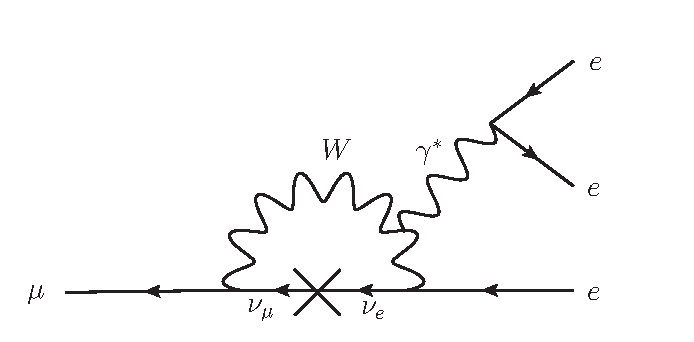
\includegraphics[width = 0.6\textwidth]{Figures/feynman_diagrams/mu_eee_SM.eps}
    \caption[$\mu^+ \rightarrow e^+ e^+ e^-$ lepton flavour violating decay through a muon neutrino oscillating to an electron neutrino.]{$\mu^+ \rightarrow e^+ e^+ e^-$ lepton flavour violating decay through a muon neutrino oscillating to an electron neutrino. This process is heavily suppressed due to the neutrino oscillation required.}
    \label{fig:mu_eee_SM}
\end{figure}
For this process, the required neutrino oscillation that mediates the lepton flavour violating component suppresses the branching ratio of this process, so much so that $\textrm{BR}(\mu^+ \rightarrow e^+ e^+ e^-) \ll 10^{-50}$.
This is an unobservably low decay rate, and so any decays of this form will almost certainly be a sign for new physics.

New physics may come in the form of new particles that can mediate these loops without a penalty as seen in the neutrino mixing, if it is to be observed.
This could be in the form of supersymmetric particles in a loop, or other particles which add couplings to muons and electrons.
It is also possible that a new light mediator adds observable contributions at tree level.

The current experimental limits on the branching ratio of various flavour violating muon decay processes are shown in Table~\ref{table:mu_br_limits}.

\begin{table}[h]
\begin{center}
\begin{tabular}{|l|l|ll|} \hline
    Decay Channel & Experiment & Branching Ratio & \\ \hline
    $\mu \rightarrow e \gamma$ & \mega & $< 1.2\times 10^{-11}$ & \cite{Brooks:1999pu} \\
                               & \meg & $< 2.4\cdot 10^{-12}$ & \cite{Adam:2011ch} \\ \hline
    $\mu \rightarrow eee$ & \sindrum & $< 1.0\times 10^{-12}$ & \cite{Bellgardt:1987du} \\ \hline
    $\mu~Au\rightarrow e~Au$ & \sindrumii & $< 7\times 10^{-13}$ & \cite{Bertl:2006up} \\ \hline
\end{tabular}
\end{center}
\caption[Branching ratio limits on muon decay from various experiments.]{Branching ratio limits on muon decay from various experiments as given in \cite{Blondel:2013ia}.}
\label{table:mu_br_limits}
\end{table}

\noindent Note that all of these upper limits are on the order of $10^{-10} - 10^{-13}$.
Any future experiments examining these decay modes must be sensitive to branching ratios at least as small as the upper limits here.
For this reason, \mueee is attempting to reach branching ratios down to $10^{-16}$ for the $\mu \rightarrow eee$ process.
To reach such a low branching ratio, at least $5.5 \times 10^{16}$ muon decays must be observed, if one assumes a total efficiency of $30\%$.

Given that this many muon decays are possible, the muon beam will be aimed at an aluminum target to stop the muons.
The decay products of the muons are then tracked with the detector.
A schematic of the target and the muon beam is shown in Fig.~\ref{fig:mu3e_target}.

\begin{figure}[h]
    \centering
    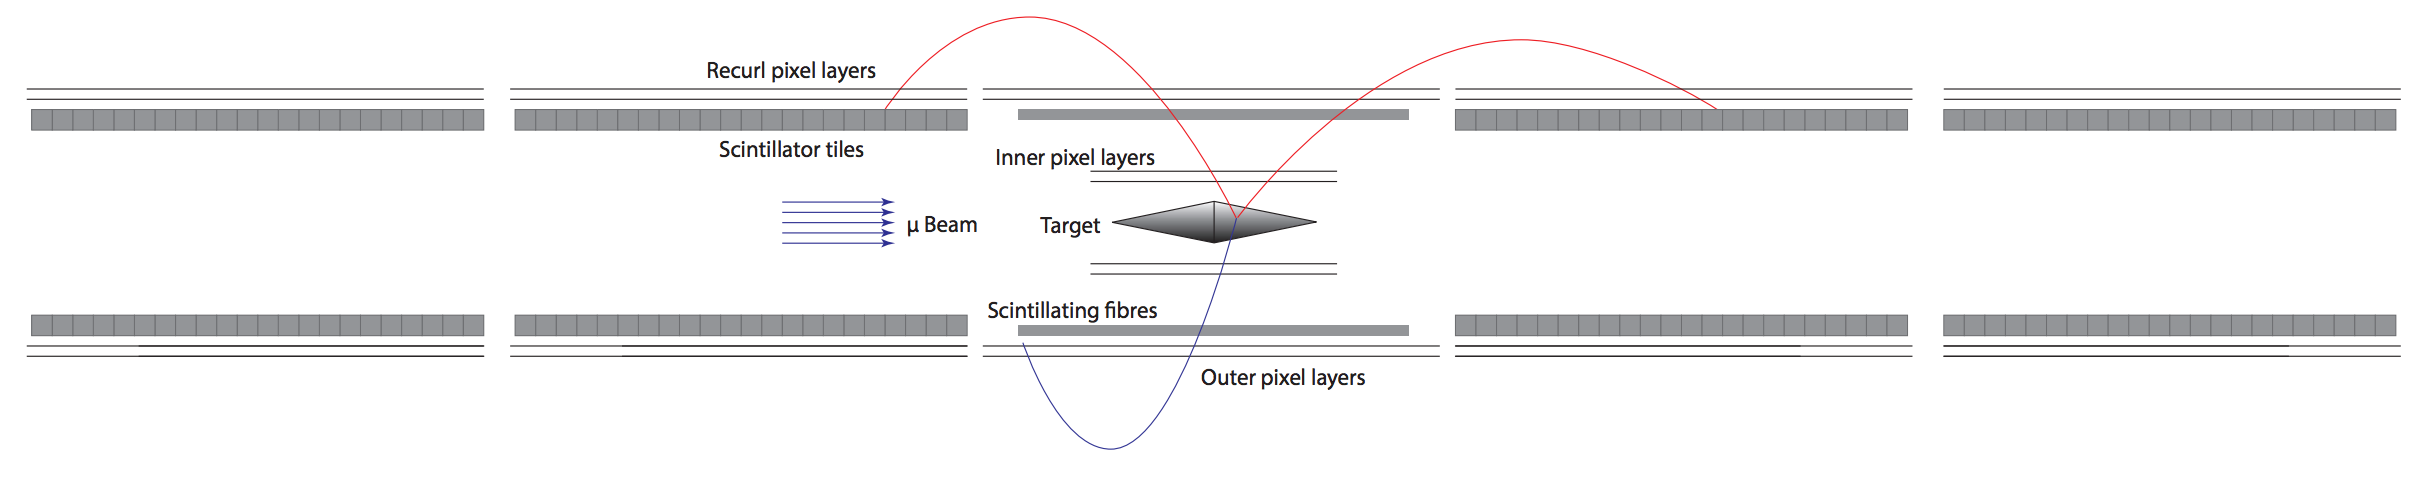
\includegraphics[width = \textwidth]{Figures/experiments/mu3e_target.png}
    \caption[Schematic of a muon decay in the full \mueee detector ready for phase II.]{Schematic of a muon decay in the full \mueee detector ready for phase II \cite{Blondel:2013ia}. The cone-shaped aluminum target can be seen in the centre with two $e^+$ tracks curling upward in red, and an $e^-$ track curling down in blue.}
    \label{fig:mu3e_target}
\end{figure}

As we will see later in this section, the energy and momentum resolution of this experiment must be excellent for it to achieve the goals specified.
This is because the SM process for $\mu^+ \rightarrow e^+ \nu_e \bar{\nu_\mu} e^+ e^-$ is much more frequent than the signal they are searching for, and rejecting this background is best done by enforcing momentum conservation to avoid missing energy in the final state.
Having excellent energy and momentum resolution is also vital for the signal we will propose, as we must have good resolution on the invariant mass of an $e^+ e^-$ pair in the final state.

In order to achieve such a low sensitivity, and for practical purposes of building and commissioning the detector, \mueee plans to run in two distinct phases of operation.
The differences between these two phases lies primarily in the differences between the beam lines, which will be discussed below.
There are also additions/modifications planned for the detector.

\subsection{Phase I}
The first phase will aim for a branching ratio sensitivity of $10^{-15}$.
PSI currently produces muons at a rate that \mueee can take advantage of for the first phase, without modifications, and the first phase can additionally serve as a commissioning time.
To produce the muons for the experiment, phase I will use the existing $\pi\textrm{E5}$ beam line.
This is done by colliding protons on the target to produce pions.
The proceeding strong interaction is given in equation~\ref{eqn:pion_production}.

\begin{equation}
\label{eqn:pion_production}
p^+ + p^+ \rightarrow p^+ + n + \pi^+
\end{equation}

\noindent Note that this process is independent of the target $Z$ since the interaction takes place directly between the proton beam and a single proton on the target.
However, a carbon target is chosen due to, among other reasons, good heat dissipation, and its high density allows for a compact target with good pion production per unit volume.
For production to be possible, the excess centre-of-mass energy must be at least as large as the pion mass, giving a threshold energy of $290~\textrm{MeV}$ for the proton beam.
To obtain a reasonable yield of pions, a $590~\textrm{MeV}$ proton beam is used that produces low energy ($10-120~\textrm{MeV}$) pions.
A beam current of $2.3\textrm{mA}$ will be used.

Pions that have stopped near the surface of the target give rise to surface muons, since the pion decays through the weak force to muons, as shown in equation~\ref{eqn:muon_production}.

\begin{equation}
\label{eqn:muon_production}
\pi^+ \rightarrow \mu^+ + \nu_\mu
\end{equation}

\noindent The pions have incredibly short lifetimes of $2.6 \times 10^{-8}~\textrm{s}$, and the branching ratio of this process is very large: $\textrm{BR}(\pi^+ \rightarrow \mu^+ + \nu_\mu) = 99.98770\%$~\cite{Agashe:2014kda}.
One does not have to wait long then to have a good source of surface muons.
A number of $10^{15}$ muon decays can be expected during this phase.
Since the decaying pions are at rest, and the muon has a mass very close to that of the pion, the muons are produced with momenta of $28~\textrm{MeV}$.
These are easy to collimate and provide a very monochromatic beam of muons, since only $10\%$ of the surface muons can be used due to an angular selection.
The collimated beam of positively charged muons is then directed to a target within a solenoidal magnetic field at a rate of $1 \times 10^8~\mu^+/\textrm{s}$.
A schematic of the beam line that produces the muon beam is shown in Fig.~\ref{fig:mu3e_phaseI_schematic}.

\begin{figure}[h]
    \centering
    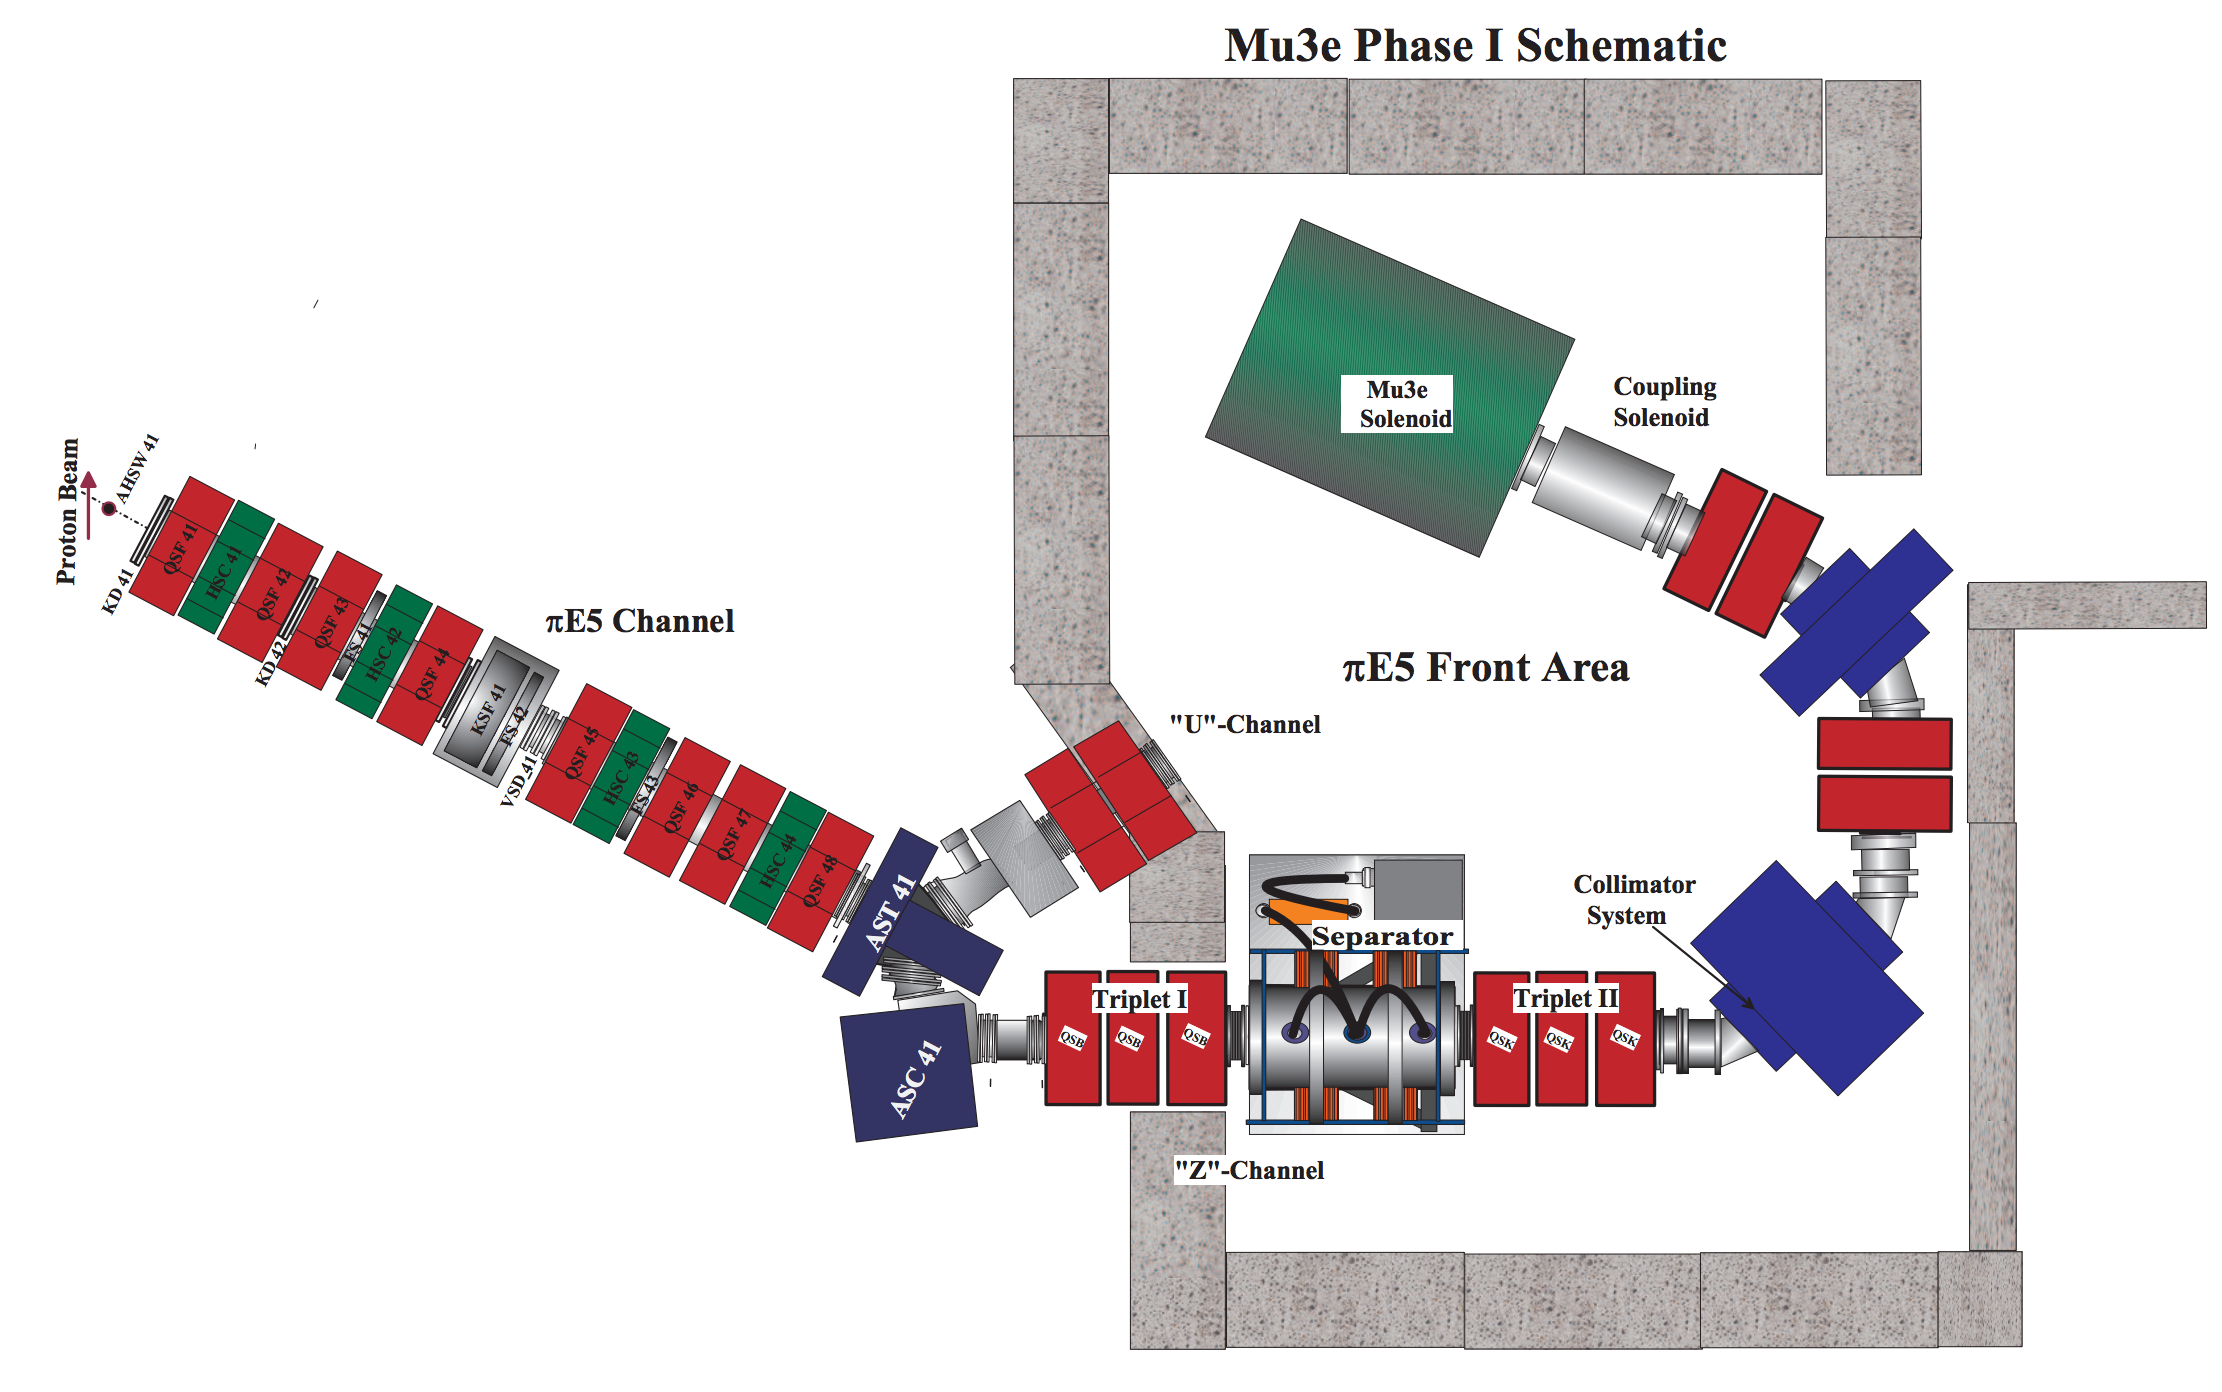
\includegraphics[width = \textwidth]{Figures/experiments/mu3e_phase1_schematic.png}
    \caption[\mueee phase I beam line schematic using the $\pi\textrm{E5}$ at PSI.]{\mueee phase I beam line schematic using the $\pi\textrm{E5}$ at PSI \cite{Blondel:2013ia}.}
    \label{fig:mu3e_phaseI_schematic}
\end{figure}

At this time, the detector is relatively minimal compared to the plan for the full run and is currently using a pixel-only detector.
The target is surrounded with a set of inner and outer silicon pixel detectors, allowing the determination of momentum, vertex position, and decay time.
Phase I is actually split into phase IA and phase IB; a detector upgrade will occur in phase IB\@.
The silicon pixel detectors used in phase IA have relatively poor momentum and timing precision and are the main focus of the upgrades.
Even so, phase IA will have sensitivity on the branching ratios down to $\order(10^{-14})$.

For phase IB, the first pair of recurl pixel layers will be added, along with the tile detectors and the fibre tracker.
The recurl stations allow for the decay products to be seen as coming from outside the detector, as the radius of the charged decay products is typically larger than the detector.
Improvements from adding the recurl stations with the tile detectors allow for momentum resolution of $0.44~\textrm{MeV}$.
Similarly, the fibre tracker and tile detector also improve the timing resolution to $\order(100-300~\textrm{ps})$. 
It is also worth noting that the total energy resolution is less than $1~\textrm{MeV}$.

\subsection{Phase II}
The largest difference between phase II and phase I is the upgrade planned for the beam line, where the $\pi\textrm{E5}$ muon beam will be replaced by the planned high-intensity muon beam (HiMB).
The HiMB will work by taking advantage of the Swiss Spallation Neutron Source (SINQ) already in place at PSI.

Similarly to the $\pi\textrm{E5}$ beam, a proton beam strikes a target, however now the target is a spallation neutron source.
As the protons strike the target, which is made of lead, zirconium, aluminum alloy, surface muons are created in the aluminum layer.
The muons that are accessible are travelling in the opposite direction of the proton, such that even though they have the same sign charge, they can be separated by bending them in opposite directions, and a collimated beam of muons can be created.
A diagram of the new beam line is shown in Fig.~\ref{fig:mu3e_phaseII_schematic}, where the \mueee detector would be placed on the far side of the muon beam cellar.

\begin{figure}[h]
    \centering
    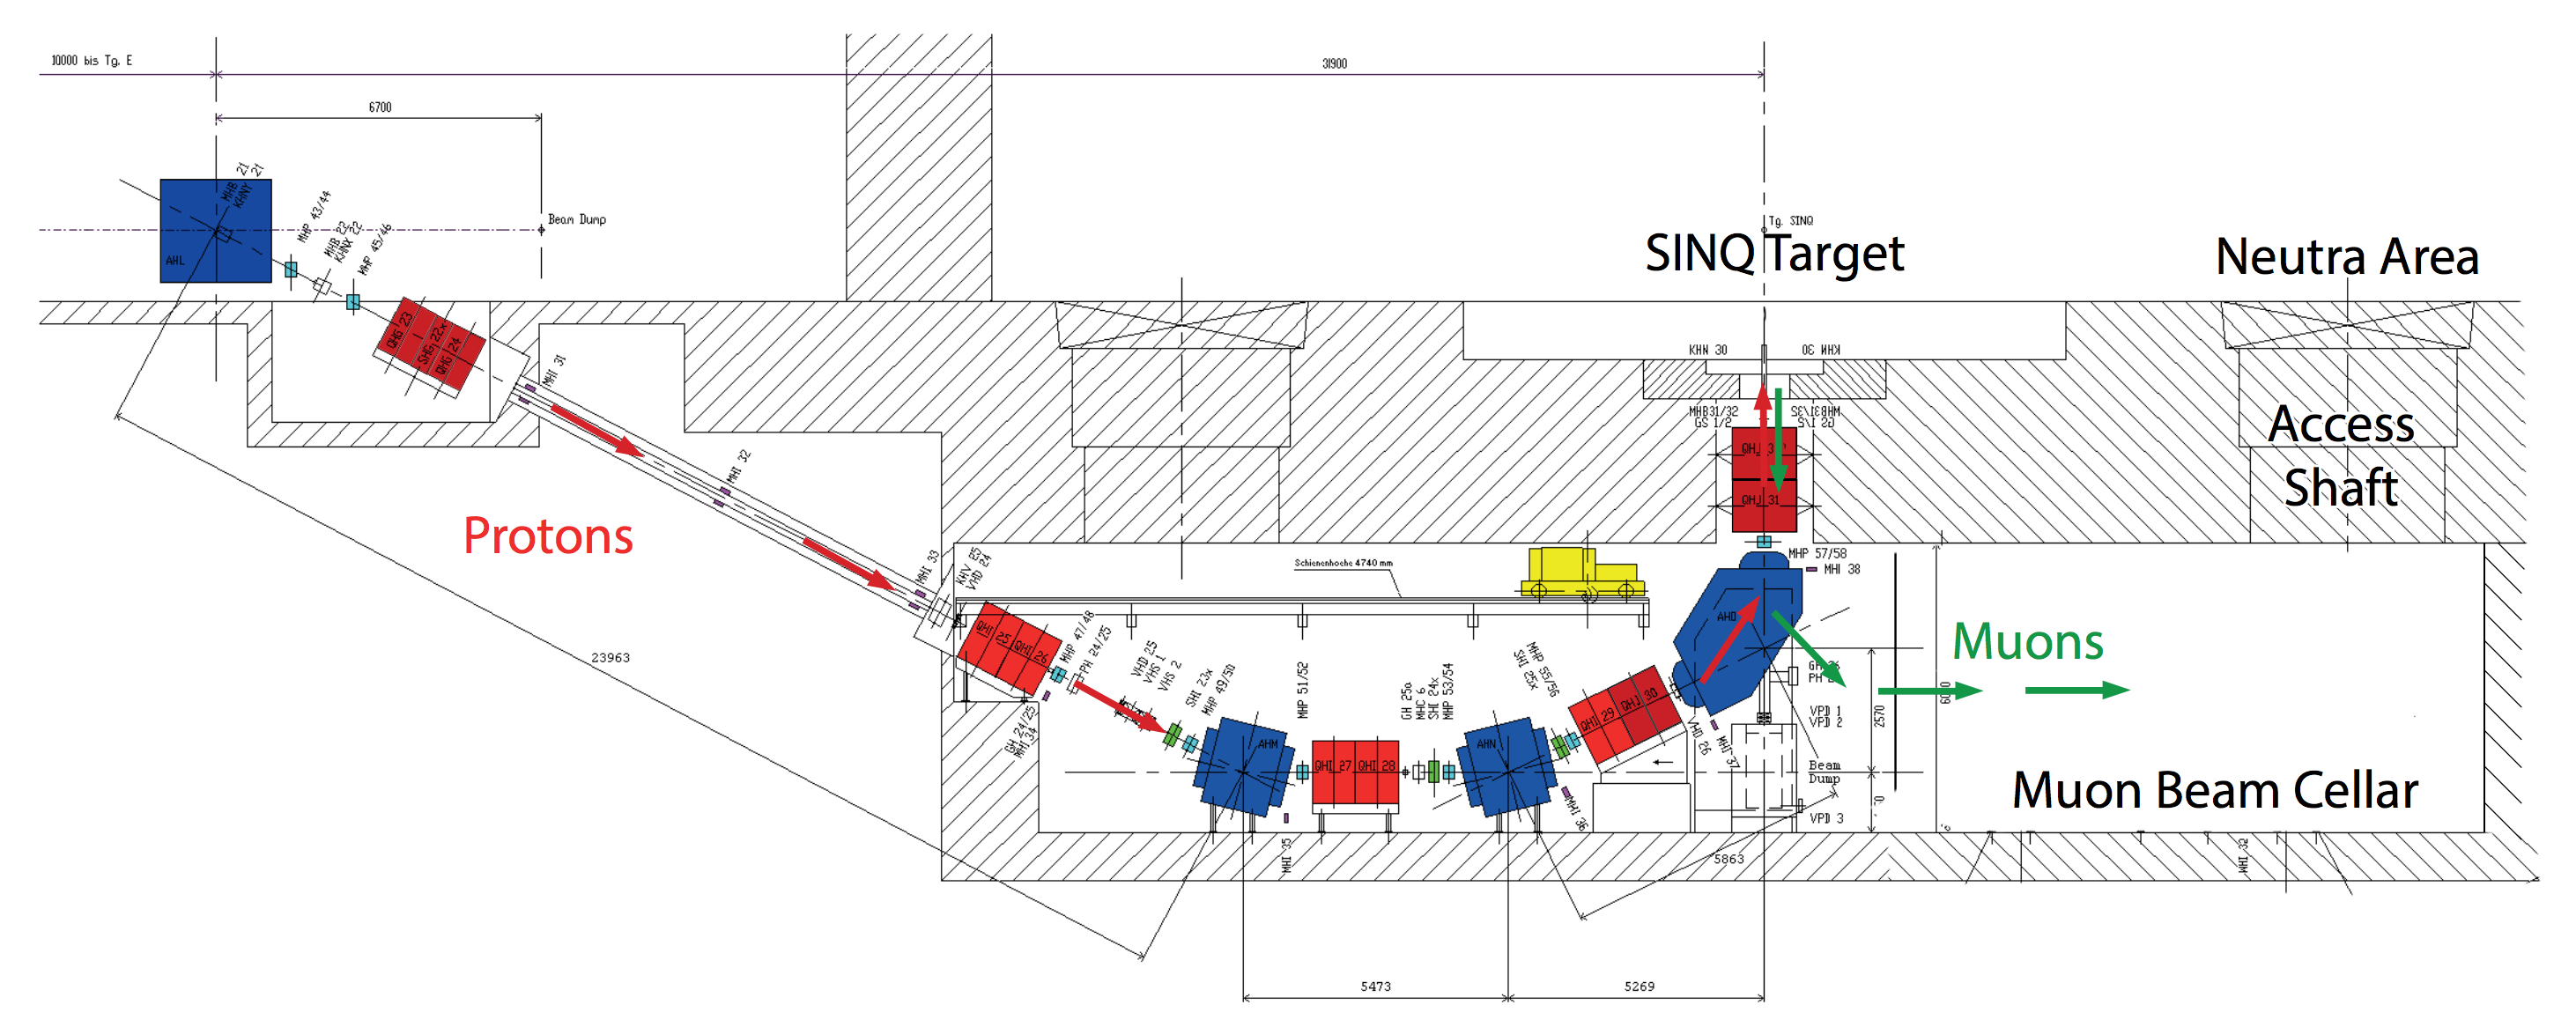
\includegraphics[width = \textwidth]{Figures/experiments/mu3e_phase2_schematic.png}
    \caption[\mueee phase II beam line schematic using the HiMB at PSI.]{\mueee phase II beam line schematic using the HiMB at PSI \cite{Blondel:2013ia}.
    The \mueee detector would be placed past the muon beam cellar.
    This production mechanism can allow for $\order(10^{10})~\mu^+/\textrm{s}$ decays.}
    \label{fig:mu3e_phaseII_schematic}
\end{figure}

Moving to the HiMB provides an estimated muon decay rate of $2 \times 10^9~\mu^+/\textrm{s}$.
To take advantage of the high-intensity beam, the detector will also receive an upgrade, where a second set of recurl stations will be added to further improve momentum resolution.
This improves the momentum resolution to $0.28~\textrm{MeV}$.

For all phases combined, the expected branching ratio sensitivities are shown in Fig.~\ref{fig:mu3e_br_limits}.
Across the entire lifetime of the experiment, it is expected to see a total of $5.5 \times 10^{16}$ muon decays for study.

\begin{figure}[h]
    \centering
    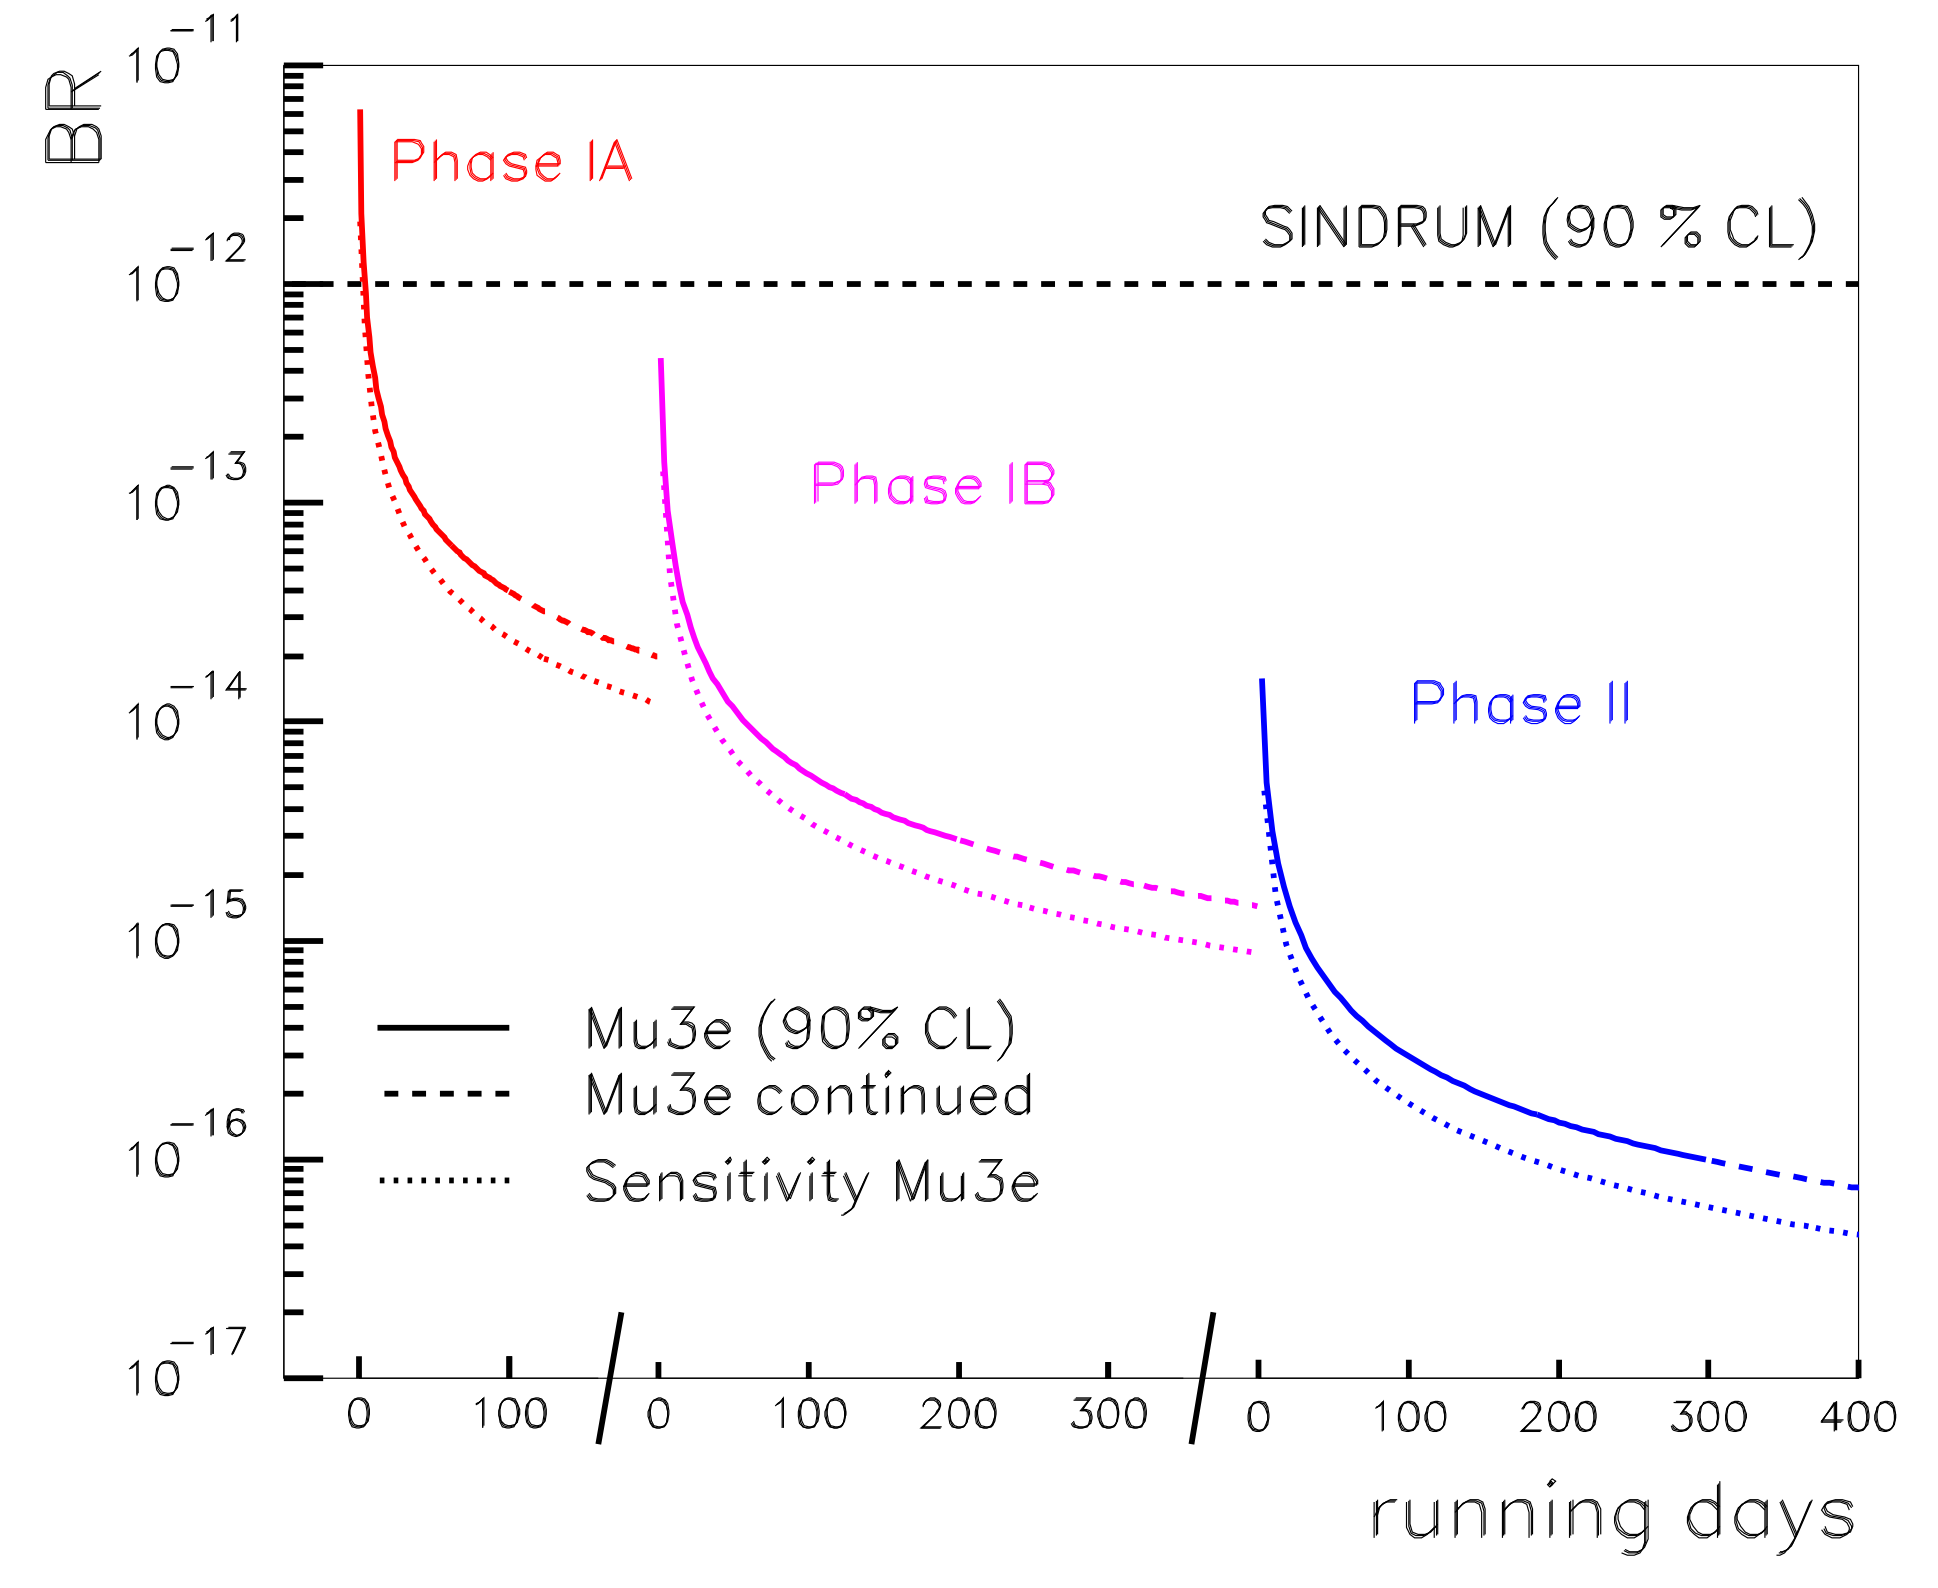
\includegraphics[width = 0.6\textwidth]{Figures/experiments/mu3e_br_limits.png}
    \caption[Expected branching ratio sensitivity for \mueee.]{Expected branching ratio sensitivity for \mueee \cite{Blondel:2013ia}.
    Each phase can be seen to distinctively increase the sensitivity, with the target sensitivity being reached with the HiMB beam line upgrades and the two recurl stations with fibre tracker being added.}
    \label{fig:mu3e_br_limits}
\end{figure}
